%&pdflatex
\documentclass[final]{beamer}

\usepackage[scale=1.24]{beamerposter} % Use the beamerposter package for laying out the poster

\usetheme{confposter} % Use the confposter theme supplied with this template

\setbeamercolor{block title}{fg=black,bg=white} % Colors of the block titles
\setbeamercolor{block body}{fg=black,bg=white} % Colors of the body of blocks
\setbeamercolor{block alerted title}{fg=white,bg=dblue!70} % Colors of the highlighted block titles
\setbeamercolor{block alerted body}{fg=black,bg=dblue!10} % Colors of the body of highlighted blocks
% Many more colors are available for use in beamerthemeconfposter.sty


\usetikzlibrary{backgrounds}
\usetikzlibrary{calc}

\usepackage{relsize}

\tikzset{fontscale/.style = {font=\relsize{#1}}
    }

\newcommand{\bigcomp}{\operatornamewithlimits{\bigcirc}}


\newlength{\sepwid}
\newlength{\onecolwid}
\newlength{\twocolwid}
\newlength{\threecolwid}
\setlength{\paperwidth}{48in} % A0 width: 46.8in
\setlength{\paperheight}{36in} % A0 height: 33.1in
\setlength{\sepwid}{0.024\paperwidth} % Separation width (white space) between columns
\setlength{\onecolwid}{0.22\paperwidth} % Width of one column
\setlength{\twocolwid}{0.464\paperwidth} % Width of two columns
\setlength{\threecolwid}{0.708\paperwidth} % Width of three columns
\setlength{\topmargin}{-0.5in} % Reduce the top margin size


\setbeamertemplate{headline}{
 \leavevmode
  \begin{columns}
  \begin{column}{.04\linewidth}
  \end{column}
     \begin{column}{.15\linewidth}
\hfill 
\includegraphics[width=1\linewidth]{logo.png} 
   \end{column}
   \begin{column}{.73\linewidth}
    \vskip1cm
    \centering
    \usebeamercolor{title in headline}{\color{jblue}\Huge{\textbf{\inserttitle}}\\[0.5ex]}
    \usebeamercolor{author in headline}{\color{fg}\Large{\insertauthor}\\[1ex]}
    \usebeamercolor{institute in headline}{\color{fg}\large{\insertinstitute}\\[1ex]}
    \vskip1cm
   \end{column}
   \begin{column}{.17\linewidth}
   \end{column}
   \vspace{1cm}
  \end{columns}
 \vspace{0.5in}
 \hspace{0.5in}\begin{beamercolorbox}[wd=47in,colsep=0.15cm]{cboxb}\end{beamercolorbox}
 \vspace{0.1in}
}

%-----------------------------------------------------------

\usepackage{graphicx}  % Required for including images

\usepackage{booktabs} % Top and bottom rules for tables

%----------------------------------------------------------------------------------------
%	TITLE SECTION 
%----------------------------------------------------------------------------------------

\title{Parameter Reduction using Generalized Neural Networks} % Poster title

\author{William Guss} % Author(s)

\institute{Machine Learning at Berkeley} % Institution(s)

%----------------------------------------------------------------------------------------

\begin{document}

\addtobeamertemplate{block end}{}{\vspace*{2ex}} % White space under blocks
\addtobeamertemplate{block alerted end}{}{\vspace*{2ex}} % White space under highlighted (alert) blocks

\setlength{\belowcaptionskip}{2ex} % White space under figures
\setlength\belowdisplayshortskip{2ex} % White space under equations

\begin{frame}[t] % The whole poster is enclosed in one beamer frame

  \begin{columns}[t]
    \begin{column}{\sepwid}\end{column} % Empty spacer column

    \begin{column}{\onecolwid} % The first column
      %!TEX root = main.tex

\begin{alertblock}{Abstract}
Classification and prediction tasks
on high resolution continuous data require models with \emph{exponentially many parameters}.
 In this paper we generalize artificial neural networks to infinite dimensional Banach spaces to attack the curse of dimensionality. Using this new class of algorithms, $\{\mathcal{G}\}$, 
we prove a new universal approximation theorem for bounded continuous operators and show that this new functional representation
of weights is invariant to the number of samples.
\end{alertblock}


\begin{block}{The Problem with High Resolution}

Computationally, we deal with \emph{discrete data}, but most of the time this data is sampled from a \emph{continuous process}. For example,
\begin{itemize}
	\item \emph{Audio}: Inherently a continuous $f: \mathbb{R} \to \mathbb{R}$ sampled as a vector $v \in \mathbb{R}^{44,100\times t}$
	\item \emph{Images}: Truthfully a function $f: \mathbb{R}^2 \to \mathbb{R}^3,$ but sampled as $v \in \mathbb{R}^{3872\times 2592}$
\end{itemize}
However, performing tractable machine learning on this data almost always requires some \emph{lossy preprocessing} like PCA or Discrete Fourier Analysis[1]. Even the state of the art approaches, convolutional neural networks, \emph{do not escape the dimensionality issues associated with high resolution data} [1,2]. \\[1cm]
\end{block}

\begin{block}{Our Solution}
\textbf{In answer to this problem, we assume the data is a continuous $f: X \to \mathbb{R}$.}
\begin{itemize}
	\item This leads to a powerful generalization of ANNs, $\{\mathcal{G}\}$ which are \emph{universal approximators of $K: L^p(X) \to L^q(X)$}
	\item Assuming continuity gives \emph{invariance to input resolution} and a \emph{massive reduction of parameters}.
\end{itemize}
\end{block}

    \end{column} % End of the first column

    \begin{column}{\sepwid}\end{column} % Empty spacer column

    \begin{column}{\twocolwid} % Begin a column which is two columns wide (column 2)
      %!TEX root = main.tex

\begin{figure}
\centering
%!TEX root = main.tex



\def\layersep{4cm}
\begin{tikzpicture}[shorten >=1pt,->,draw=black!90, node distance=\layersep]


    \tikzstyle{every pin edge}=[<-,shorten <=1pt]
    \tikzstyle{neuron}=[circle,fill=black!25,minimum size=50pt,inner sep=0pt]
    \tikzstyle{input neuron}=[neuron, fill=red!50];
    \tikzstyle{output neuron}=[neuron, fill=blue!50];
    \tikzstyle{hidden neuron}=[neuron, fill=black!50];
    \tikzstyle{annot} = [text width=4em, text centered]

    % Draw the input layer nodes
    \foreach \name / \y in {1,...,2}
    % This is the same as writing \foreach \name / \y in {1/1,2/2,3/3,4/4}
        \node[input neuron, pin=left: \(x_\y\)] (I-\name) at (0,-\y in) {};

    % Draw the hidden layer nodes
    \foreach \name / \y in {1,...,3}
        \path[yshift=0.5cm]
            node[hidden neuron] (H1-\name) at (\layersep,-\y in) {};
            
     \foreach \name / \y in {1,...,3}
        \path[yshift=0.5cm]
            node[hidden neuron] (H2-\name) at (2*\layersep,-\y in) {};

    % Draw the hidden layer nodes
    \foreach \name / \y in {1,...,2}
        \path[yshift=0.5cm]
            node[output neuron, pin=right:\(\sigma_{\name}^{(3)}\)] (O-\name) at (3*\layersep,-1cm -\y in) {};


    % Connect every node in the input layer with every node in the
    % hidden layer.
    \foreach \source in {1,...,2}
        \foreach \dest in {1,...,3}
            \path (I-\source) edge (H1-\dest);

    % Connect every node in the hidden layer with the output layer
    
        \foreach \source in {1,...,3}
        \foreach \dest in {1,...,3}
        \path (H1-\source) edge (H2-\dest);
    \foreach \source in {1,...,3}
        \foreach \dest in {1,...,2}
        \path (H2-\source) edge (O-\dest);

    \node[annot] at (6,0) {\(\mathcal{N(\pmb{x})}}\)};


   \node[circle, minimum size=50pt, inner sep=0pt, pin=left: \(x_\infty\), fill=red!50] (i0) at (0,-4 in) {$\infty$};

   \node[circle, inner sep=0pt, minimum size=50pt, fill=black!50] (i1) at (1*\layersep,-4 in) {$\infty$};

   \node[circle, inner sep=0pt, minimum size=50pt, fill=black!50] (i2) at (2*\layersep,-4 in) {$\infty$};

   \node[circle, inner sep=0pt, minimum size=50pt, fill=blue!50, pin=right:\(\sigma_{\infty}^{(3)}\)] (i3) at (3*\layersep,-4 in) {$\infty$};


    \begin{scope}[on background layer]
		 \draw[loosely dotted, color=black, line width=0.7mm] (I-2) --   (i0);
		 \draw[loosely dotted, color=black, line width=0.7mm] (H1-3) --   (i1);
		 \draw[loosely dotted, color=black, line width=0.7mm] (H2-3) --   (i2);
		 \draw[loosely dotted, color=black, line width=0.7mm] (O-2) --   (i3);


		\foreach \source in {1,...,2}
		    \draw[loosely dotted, color=black!30, line width=0.5mm]  (I-\source) -- (i1);
		\foreach \dest in {1,...,3}
		    \draw[loosely dotted, color=black!30, line width=0.5mm] (i0) -- (H1-\dest);
		\foreach \source in {1,...,3}
		    \draw[loosely dotted, color=black!30, line width=0.5mm]  (H1-\source) -- (i2);

    	\foreach \dest in {1,...,3}
		    \draw[loosely dotted, color=black!30, line width=0.5mm] (i1) -- (H2-\dest);

		\foreach \source in {1,...,3}
		    \draw[loosely dotted, color=black!30, line width=0.5mm]  (H2-\source) -- (i3);

    	\foreach \dest in {1,...,2}
		    \draw[loosely dotted, color=black!30, line width=0.5mm] (i2) -- (O-\dest);


	 \end{scope}


	 %%% The next part of the image.
	 %\node[annot, fontscale=4] at (\layersep*4.25, -2.5 in) {$\cong$};



	\draw[fill=red!50]  (\layersep*6 +0.7cm, -2.5 in) -- +(\layersep/2, 2 in) -- +(\layersep/2, -2in) -- cycle;
	\draw (\layersep*6 +0.7cm + \layersep/2, -.5 in) -- +(\layersep/2, 0in) --  +(\layersep/2, -4 in) -- +(0, -4 in) -- cycle;
	\draw[fill=black!70] (\layersep*6 +0.7cm + \layersep, -.5 in)  -- +(\layersep/2, -2 in) -- +(0, -4in) -- cycle;
	\node[annot] at (\layersep*6.75 +0.7cm, -2.5 in)  {$T_1$};

		\draw[fill=black!70]  (\layersep*7.5 +0.7cm, -2.5 in) -- +(\layersep/2, 2 in) -- +(\layersep/2, -2in) -- cycle;
	\draw (\layersep*7.5 +0.7cm + \layersep/2, -.5 in) -- +(\layersep/2, 0in) --  +(\layersep/2, -4 in) -- +(0, -4 in) -- cycle;
	\draw[fill=black!70] (\layersep*7.5 +0.7cm + \layersep, -.5 in)  -- +(\layersep/2, -2 in) -- +(0, -4in) -- cycle;
	\node[annot] at (\layersep*8.25 +0.7cm, -2.5 in)  {$T_2$};

	\draw[fill=black!70]  (\layersep*10 +0.7cm -0.4cm , -2.5 in) -- +(\layersep/2, 2 in) -- +(\layersep/2, -2in) -- cycle;
	\draw (\layersep*10 +0.7cm -0.4cm  + \layersep/2, -.5 in) -- +(\layersep/2, 0in) --  +(\layersep/2, -4 in) -- +(0, -4 in) -- cycle;
	\draw[fill=blue!50] (\layersep*10 +0.7cm -0.4cm  + \layersep, -.5 in)  -- +(\layersep/2, -2 in) -- +(0, -4in) -- cycle;
	\node[annot] at (\layersep*10.75 +0.7cm -0.4cm , -2.5 in)  {$T_L$};



	 \node[circle, inner sep=0pt] (xi) at (\layersep*6 -0.7cm, -2.5 in)  {$\xi$};
	 \path (xi) edge (\layersep*6 +0.7cm, -2.5 in);

	\node[circle, fill=white, draw, fontscale=-1, inner sep=3pt] at (\layersep*6.5 +0.7cm + \layersep, -2.5 in) {$g$};

	\node[circle, fill=white, draw, fontscale=-1, inner sep=3pt] at (\layersep*8 +0.7cm + \layersep, -2.5 in) {$g$};

	\node[annot] at (\layersep*8.5 +0.5cm + \layersep, -2.5 in) {$\ldots$};


	\node[circle, fill=white, draw, fontscale=-1, inner sep=3pt] at (\layersep*9 +0.3cm + \layersep, -2.5 in) {$g$};

	\node[circle, inner sep=0pt] (out) at (\layersep*11 +0.3cm + \layersep, -2.4 in) {$\sigma^{(L)}$};
	 \path  (\layersep*11.75, -2.5 in) edge (\layersep*11.5, -2.5 in);


    \node[annot] at (\layersep*9,0) {\(\mathcal{G}(\pmb{\xi})\)};
\end{tikzpicture}
\caption{Left: A neural network $\mathcal{N}$ as the number of nodes $\to \infty.$ Right: 
A generalized neural network $\mathcal{G}.$}
\end{figure}


\begin{columns}[t,totalwidth=\twocolwid] % Split up the two columns wide column

\begin{column}{\onecolwid}\vspace{-.6in} % The first column within column 2 (column 2.1)

	\begin{block}{Operator Neural Networks}
	 	\textbf{Definition 1.}
	    \emph{We say $\mathcal{N}: \mathbb{R}^n \to \mathbb{R}^m$ is a feed-forward neural network if for an input vector $\pmb{x}$,}
	        \begin{equation}
	                \begin{aligned}
	            \mathcal{N}:\ & \sigma_j^{(l+1)} = g\left(\sum_{i}w_{ij}^{(l)}\sigma_i^{(l)} + \beta^{(l)}\right) &\\  & \sigma_i^{(0)} \ \ \ =x_i.& 
	            \end{aligned}
	        \end{equation}
	         \emph{Furthermore we say $\{\mathcal{N}\}$ is the set of all neural networks.}


	      \begin{equation*}
			\Big\Downarrow      
	      \end{equation*}

	     \textbf{Definition 2. }\emph{We call $\mathcal{O}: L^p(X) \to L^q(Y)$ an operator neural network if,}
		\begin{equation}
	          \begin{alignedat}{2}
	        \mathcal{O}:\ &\sigma^{(l+1)}(j) & &=  g\left(\int_{X} \sigma^{(l)}(i) w^{(l)}(i,j)\ di \right)  \\
	        &\sigma^{(0)}(i) & &= f(i). 
	        \end{alignedat}
		\end{equation}
		\emph{Furthermore let $\{\mathcal{O}\}$ denote the set of all operator neural networks.}
	\end{block}


\end{column} % End of column 2.1


\begin{column}{\onecolwid}\vspace{-.6in} % The second column within column 2 (column 2.2)


\begin{block}{Layer Types}
	We suggest several types of layers in the category. \\
    $\;\;T_l$ is \emph{$\mathfrak{o}$-operational} if
     \begin{equation} \label{eq:tlfunctional}
    \begin{aligned} 
       \mathfrak{o}: L^p(X}) \to&\ L^q(Y}) \\
      \sigma \mapsto& \int_{X} \sigma(i) w^{(l)}(i,j)\ di.
    \end{aligned}
    \end{equation}
   $\;\;T_l$ is \emph{ $\mathfrak{n}$-discrete } if
    \begin{equation} \label{eq:tldiscrete}
    \begin{aligned} 
       \mathfrak{n}: \mathbb{R}^n \to&\ \mathbb{R}^m \\
      \vec{\sigma} \mapsto& \sum_j^m \vec{e}_j\sum_i^n \sigma_i w^{(l)}_{ij}
    \end{aligned}
    \end{equation}
     $\;\;T_l$ is \emph{$\mathfrak{n}_1$-transitional } if
    \begin{equation} \label{eq:tldiscrete}
    \begin{aligned} 
       \mathfrak{n}_1: \mathbb{R}^n \to&\  L^q(Y) \\
      \vec{\sigma} \mapsto& \sum_i^n \sigma_i w^{(l)}_i(j).
    \end{aligned}
    \end{equation}
    $\;\;T_l$ is \emph{$\mathfrak{n}_2$-transitional } if
    \begin{equation} \label{eq:tldiscrete}
    \begin{aligned} 
       \mathfrak{n}_2: L^p(X) \to&\ \mathbb{R}^m \\
      \sigma(i) \mapsto& \sum_j^m \vec{e}_j\int_{X} \sigma(i) w^{(l)}_j(i)\ di
    \end{aligned}
    \end{equation}
\end{block}



\end{column}

\end{columns}




\begin{columns}[t,totalwidth=\twocolwid] % Split up the two columns wide column

\begin{column}{\onecolwid}\vspace{-.6in} % The first column within column 2 (column 2.1)

	\begin{block}{Generalized Neural Networks}

	{Both $\mathcal{O}$ and $\mathcal{N}$ look really similar. Is there some more general category or structure containing them?} \\[0.7cm]

	\textbf{Definition 3.} \emph{If $A,B$ are (possibly distinct) Banach spaces over a field $\mathbb{F}$,
		we say $\mathcal{G}: A \to B$ is a generalized neural network if and only if }
	\begin{equation} \label{eq:gann}
	          \begin{alignedat}{2}
	        \mathcal{G}:\ &\sigma^{(l+1)} & &=  g\left(T_l\left[\sigma^{(l)}\right] + \beta^{(l)}\right)  \\
	        &\sigma^{(0)} & &= \xi 
	        \end{alignedat}
	\end{equation}
	\emph{for some input $\xi \in A$, and a linear form $T_l$. Denote the set of all such networks, $\{\mathcal{G}\}$} \\[0.7cm]
	\textbf{Remark.} \mathcal{G} is a \emph{category}, and we can write neural networks as \emph{commutative diagrams}.
	\end{block}
\end{column}


\begin{column}{\onecolwid}\vspace{-.6in} % The first column within column 2 (column 2.1)

\begin{block}{ANNs as Commutative Diagrams}
This generalization is nice from a creative standpoint. We make new "classifiers" as we like. \\

	\textbf{Examples:}
	\begin{itemize}
		\item A three-layer neural network is just
		\begin{equation*}
			\mathcal{N}_3: \mathbb{R}^{10000} \xrightarrow{g \circ \mathfrak{n}}\mathbb{R}^{30}  \xrightarrow{g \circ \mathfrak{n}} \mathbb{R}^{3}.
		\end{equation*}
		\item A three-layer operator network is simply
		\begin{equation*}
			\mathcal{O}_3: L^p(R) 	 \xrightarrow{g \circ \mathfrak{o}} L^1(R) \xrightarrow{g \circ \mathfrak{o}} C(R).
		\end{equation*}
		\item We can even classify functions!
		\begin{equation*}
			\mathcal{C}:  L^p(X) 	 \xrightarrow{g \circ \mathfrak{o}} L^1(X)  \xrightarrow{g \circ \mathfrak{o}} L^1(X)\xrightarrow{g \circ \mathfrak{n}_2}  \mathbb{R}^n.
		\end{equation*}
	\end{itemize}
\end{block}

\end{column}

\end{columns}

    \end{column}

    \begin{column}{\sepwid}\end{column} % Empty spacer column

    \begin{column}{\onecolwid} % The third column
      %!TEX root = main.tex

\setbeamercolor{block alerted title}{fg=black,bg=norange} % Change the alert block title colors
\setbeamercolor{block alerted body}{fg=black,bg=black!4} % Change the alert block body colors


\begin{alertblock}{Results}
	
 \textbf{Theorem 1. (Inclusion)} It follows that $$\{\mathcal{N}\} \subset \{\mathcal{O}\} \subset \{\mathcal{G}\}.$$ \\
 \setlength\parindent{24pt}
 \indent Inclusion is the first and most important result to this generalization. For every $\mathcal{N}$ there exists an $\mathcal{O}$ such that $\mathcal{O} \simeq \mathcal{N}.$ \\[0.7cm]
  \setlength\parindent{0pt}


  \textbf{Theorem 2. (Universality) } Let $F: A \to B$ be a continuous operator between Banach spaces. For every $\epsilon > 0$, there exist a GANN
$$  \mathcal{G}_2: A 	 \xrightarrow{g \circ T_1} C \xrightarrow{g \circ T_2} B$$
such that for all $\xi$
$$ \| {C}(\xi) -  F(\xi) \| < \epsilon.$$ \\[0.7cm]


	\begin{figure}
		 	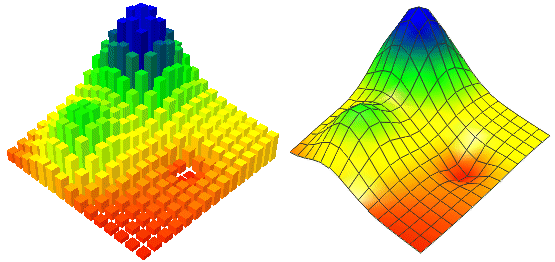
\includegraphics[width=0.6\onecolwid]{gc082_1.png}
		 	\caption{Parameter reduction using weight polynomials.}
	\end{figure}

\textbf{Theorem 3. (Parameter Reduction)} 
Let $\mathcal{C}$ be a continuous classifier
$$\mathcal{C}:  L^p(X) 	 \xrightarrow{g \circ \mathfrak{o}} L^q(Y) \xrightarrow{g \circ \mathfrak{n}_2}  \mathbb{R}^n.$$ with $O(1)$ weight polynomials.  If a continuous function, say $f(t)$ is sampled uniformly from $t = 0$, to $t = N$, such that $x_n = f(n)$,  then there exists a unique $\mathcal{N} \simeq \mathcal{C}$ with  $O(N^2)$ weights. \\[0.7cm]

\textbf{Generalized Backpropagation.} If $\mathcal{G}$ is parameterized by $W^{l} \in \mathbb{R}^{n\times m}$ then
\begin{equation*}
	B \otimes A \ni \frac{\partial \mathcal{G}}{\partial W^l} =
	   \underbrace{\left[\bigcomp_{k=L}^{l}  Dg \circ T_k\right]}_{\delta_{l+1}\text{ from BP}} \circ Dg \circ D\pi_l.
\end{equation*}

\end{alertblock}	


\begin{block}{References}
\footnotesize{
    \begin{thebibliography}{99} % Beamer does not support BibTeX so references must be inserted manually as below
        \bibitem[1]{p1} Burch, Carl (2012)
        \newblock A survey of machine learning
        \newblock \emph{International Conference on Artificial Intelligence and Statistics}
        \bibitem[2]{p1} Roux, Nicolas L and Bengio, Yoshua (2007)
        \newblock Continuous Neural Networks
        \newblock \emph{Journal of Machine Learning Research}
        
    \end{thebibliography}
}


 \end{block}

    \end{column} % Endz of the third column


  \end{columns}


\end{frame} % End of the enclosing frame

\end{document}
